\documentclass{article} % For LaTeX2e
\usepackage{nips15submit_e,times}
\usepackage{hyperref}
\usepackage{url}
%\documentstyle[nips14submit_09,times,art10]{article} % For LaTeX 2.09

\usepackage{graphicx}
\usepackage{subfigure}
\usepackage{algorithmic}
\usepackage{algorithm}
\usepackage{amsmath}
\usepackage{multirow}
\usepackage{amssymb}
% \usepackage{wrapfig,lipsum,booktabs}
\usepackage{wrapfig}

%\usepackage{etoolbox}
%\patchcmd{\thebibliography}{\section*{\refname}}{}{}{}

\title{Clustering Players Time-Series Data: A Case Study}

\author{
Yuanli Pei\thanks{This work was done while Yuanli Pei and Moises Goldszmidt were at Zynga Inc.} \\
Oregon State University, Corvallis, OR\\
\texttt{peiy@eecs.oregonstate.edu} \\
\And
Amy Tan\\
Zynga Inc., San Francisco, CA\\
\texttt{atan@zynga.com} \\
\AND
Moises Goldszmidt$^\ast$ \\
Samsung Research America, Mountain View, CA \\
\texttt{m.goldszmidt@samsung.com} \\
\And
Alexandros Ntoulas\\
Zynga Inc., San Francisco, CA \\
\texttt{antoulas@zynga.com} 
}


% \author{
% David S.~Hippocampus\thanks{ Use footnote for providing further information
% about author (webpage, alternative address)---\emph{not} for acknowledging
% funding agencies.} \\
% Department of Computer Science\\
% Cranberry-Lemon University\\
% Pittsburgh, PA 15213 \\
% \texttt{hippo@cs.cranberry-lemon.edu} \\
% \And
% Coauthor \\
% Affiliation \\
% Address \\
% \texttt{email} \\
% \AND
% Coauthor \\
% Affiliation \\
% Address \\
% \texttt{email} \\
% \And
% Coauthor \\
% Affiliation \\
% Address \\
% \texttt{email} \\
% \And
% Coauthor \\
% Affiliation \\
% Address \\
% \texttt{email} \\
% (if needed)\\
% }

% The \author macro works with any number of authors. There are two commands
% used to separate the names and addresses of multiple authors: \And and \AND.
%
% Using \And between authors leaves it to \LaTeX{} to determine where to break
% the lines. Using \AND forces a linebreak at that point. So, if \LaTeX{}
% puts 3 of 4 authors names on the first line, and the last on the second
% line, try using \AND instead of \And before the third author name.

\newcommand{\fix}{\marginpar{FIX}}
\newcommand{\new}{\marginpar{NEW}}

\nipsfinalcopy % Uncomment for camera-ready version

\begin{document}


\maketitle

\begin{abstract}
%The game industry plays an important in improving our entertainment in digital life.  One 
of the main tasks for the game companies is to develop user-specific features to 
improve their gaming experience. The key factor is to understand player's behaviors during their 
game-play. This paper  considers the following two tasks: 
Given user's time series behavior data, 1) what are the underlying playing states that 
controls user's behaviors at each time period, and 2) what are the natural groups of players based 
on their state transitions. We apply Hidden Markov Model (HMM) to identify gamers' 
hidden playing states, and use a Dirichlet clustering method to find player groups based on 
their state transitions. Our case study on one of the strategy game developed by Zynga Inc.\  
reveals interesting results that can help gamer designers to improve the game.





The game industry presents a very interesting source of challenges to machine learning methods and algorithms.  Games continuously collect data about the basic actions of players, and from that raw data, companies would like to extract actionable information to both delight players with better game experiences, and improve business metrics. In this paper we explore an approach to address a key enabler to understand players' behaviors. Given the players time series with raw data about  their  actions, (1) what are the latent states that govern that behavior, and (2) what are the natural clusters of players given the latent state dynamics.   Out approach is based on using Hidden Markov Models (HMMs) to identify the basic players latent states, and then use a clustering method based on Dirichlet Process to group the players according to the time series of these latent states. We present our preliminary results on real data taken from  one of the strategy games developed by Zynga Inc.\  




\end{abstract}


\section{Introduction}
%\input{intro.tex}
The game industry is steadily gaining grounds in the competition for our digital time. Besides the traditional economic and business analysis reports, evidence of this fact, is the declared interest of companies like Amazon (purchased Twitch), Sonny (playsattion, Microsoft (XBOX), among others.  Games are also an incredibly rich source of data about human behavior ranging from social interactions to economical and rational decision making.

From the points of view of  improving the players' experience  and also from the business aspects of retention, engagment  and payments,  it is very important for game companies to understand  player's behaviors and take appropriate actions accordingly. As players change their playing strategies and patterns during their involvement with the game (which can take years), and as these patterns are clearly not independent from previous playing behavior, the proper analysis of these patterns should be done by looking at the time series of the players actions.  These time series are multivariate in nature, as players can take over hundreds of actions in some of these games, and these actions are further parameterized by real values.

In this paper we explore an approach to characterizing players behavior from the multivariate time series of their raw actions in the game based on 
1) inducing a time series of latent states that abstract their raw actions and 2) clustering these time series of latent states.  To induce the time series of latent states we rely on  Hidden Markov Model (HMM) \cite{hmm}, with the playing states as 
the hidden nodes and the players' action statistics at each time period as the observed features.  We fit the HMM model and induce the latent  states by applying the Viterbi decoding algorithm.  We then find the groupings of players using an unsupervised clustering method based on modeling this grouping as a Bayesian version of a Dirichlet Process~\cite{}.

We test this approach on a mobile strategy game developed by Zynga Inc. %, named {\it Empires and Allies}. 
Our method found three basic latent  states generating all the raw actions, and  the clustering results reveal three 
interesting groups that contains players with similar patterns of transition states within each group.
% this needs to be strengthen...
As we will argue these results greatly simplify the task of  understanding players' behaviors to improve the game design and other business metrics as monetization and engagement. This characterization enables the game designers and managers to track and identify on a weekly basis the changes in behavior and how it correlates to changes in design, reaction to incentives, and A/B testing.  




%\section{Related Work}
%There exists a few work on clustering time series data with HMM model, such as
\cite{Bicego2006,bicego2003,coviello2014}. Most of the work focus on finding
out the final clustering result, while we are also interested in studying
the underlying states of each player at each time period. To our knowledge, 
we are not aware of any work on clustering time series data in the game domain.
The most related work in the game domain is \cite{menendez2014},
where gamers' time series data are used to extract the user profile.
However, the task considered there is different with our paper.



\section{Method}
Let $X_{it} = [X_{it1}, \cdots, X_{itD}]^\top$ be the measurements of player $i$ at the $t$-th time epoch, 
where $D$ is the number of features.  We assume that time is discrete and advances in epochs. 
The measurements of player $i$ from $t = 1$ to  $t = T$, i.e. its time series of actions in the game,  is denoted as $X_{i} = [X_{i1}, \cdots, X_{iT}]^\top$. The time series of data for   $N$ players, is denoted by $X = \{ X_1, \cdots, X_N \}$.  We remark that for different users, the total time epochs may not be the same; for simplicity of exposition, in this paper we assume  
that the time series for all users are of the same length.

{\bf Modeling Latent Players States with HMMs.}
We assume that there is a latent playing state that controls user's€™ behavior at each time period, and that furthermore the state evolves  as the player changes his strategy overtime.  We represent each players' data using a Hidden Markov Model (HMM) \cite{hmm} chain with length $T$, the total time epochs.  Let $Y_{it}$ be the hidden state representing 
the $i$-th gamer's  latent state at time $t$, and $Y_{it}$ will be regarded as discrete taking on $S$ values $\{1, \cdots, S\}$. 

%The gamer's HMM model has three parameters: 1) the initial state distribution vector $\pi$ 
%with $\pi_s$ being the probability of a gamer starting with state $s$; 
%2) the state transition parameter $A$, with $A_{rs}$ being the probability of a gamer transitioning from state
%$r$ at time $t-1$ to state $s$ at time $t$. 3) the emission parameter $B$, with $B_s$ controlling the probability of observing $X_{it}$ at state $Y_{it} = s$. 

%mpg;  These people will know what an HMM is.  So we can simplify this explanation if we need space.
The mechanism of the players HMM model is as follows: 1) initially, a player starts with state 
$Y_{i1} \in \{1, \cdots, S\}$ according to an initial distribution $\pi$,  with $\pi_s$ being 
the probability of starting at state $s$; 2) all the $Y_{it}$'s  evolves according to the 
{\it Markov property}: given $Y_{i{t-1}}$, the state $Y_{it}$ is independent of all the 
states prior to $t-1$, and the transition matrix is $A$, with $A_{rs}$ being the probability of 
transitioning from state $r$ to state $s$; 3) at each time $t$, the observations $X_{it}$ only 
depends on the state $Y_{it}$ parametrized by $B$, with $B_s$ controlling the probability 
of observing $X_{it}$ at state $Y_{it} = s$. 
Given the observed data $X$ and the number of states $S$, we  estimate the parameters, i.e., the transition matrix $A$, the emission matrix $B$, and the initial distribution $\pi$ by maximizing the 
likelihood of the observations. As usual, the free parameter $S$ is fitted via a scoring function,  In this work we rely on  BIC \cite{bic}.

%\[ \max_{\pi, A, B} P(X | \pi, A, B) = \prod_{i=1}^N P(Y_{i1} | \pi) P(X_{i1} | Y_{i1}, B) \prod_{t=2}^T P(Y_{it} | Y_{i{t-1}}, A) P(X_{it} | Y_{it}, B) ~.\]
%As usual the parameter $S$ is unknown. In this work we use the BIC criteria to fit it.
%% mpg: we need to commit to one We will estimate $S$ using criteria such as changes of data likelihood, AIC or BIC. 
 
After estimating the parameters, we find the state sequence $Y_{i1}, \cdots, Y_{iT}$  
for each user by maximizing $P(Y_{i1}, \cdots, Y_{iT}| X, \pi, A, B)$ using the  Viterbi  algorithm \cite{hmm}. 
%One possible solution is to estimate $Y_{it}$ individually by maximizing $P(Y_{it}| X_{it}, \pi, A, B)$.

{\bf Clustering Players Behavior.}
 Our  approach to clustering consists in  adapting the method proposed in~\cite{moises}, as they also looked at clustering time series of integer data (albeit in a completely different domain). We adopt the mixture of Dirichlet process model (DP) for clustering \cite{dpclustering}.  Thus, We assume the clusters evolve according to a Dirichlet distribution with parameter $\alpha$.

Let $Y = [Y_1, \cdots, Y_N]^\top$ be the state transitions for all the players,
where $Y_i = [Y_{i1}, \cdots, Y_{iT}]^\top$ denotes the $i$-th player's states from 1 to
the $T$-th time. As it is common in this approach we us $Z_i$ as an auxiliary variable denoting the  cluster assignment for the $i$-th player.  We use  $K$ be the total number of (unknown) clusters.  Again, given our model, the number of clusters will be fitted automatically as part of the model, and will be continuously updated as we collect more data. 

%{\bf The Clustering Model:}


We assume that each cluster $k$ generates a Markov chain parametrized by $\{\lambda^k, \Phi^k\}$, 
where $\lambda^k$ is the $S\time 1$ vector for the initial state distribution, 
and $\Phi^k$ is the $S \times S$ transition matrix. We use the prior distribution 
for parameters in each cluster $G_0(\{\lambda^k, \Phi^k\}) = Dir(\hat\pi) \prod_{s=1}^S Dir (\hat B_{s.})$,
where $\hat\pi$ and $\hat B$ are the estimated parameters at the first step. 
The conditional probability  
\begin{equation}
\label{eq:condi}
  P(\{\lambda^k, \Phi^k \}_{k=1}^K | Z ) 
= \prod_k G_0(\{\lambda^k, \Phi^k\})~.
\end{equation}
%The data generation process is assumed as below \\
%\begin{tabular}{l}
%    \quad For each player $i$,\\
%    \qquad 1. Sample cluster assignment $Z_i \sim Dir(\alpha)$  \\
%    \qquad 2. Generate the state sequence $Y_{i1}, \cdots Y_{iT}$ with Markov chain parametrized by $\{\lambda^{Z_i}, \Phi^{Z_i}\}$.
%\end{tabular}
Given the clustering model, the likelihood of the data of state transitions for all players is
\begin{equation}
\label{eq:likeli}
  P(Y| Z, \{\lambda^k, \Phi^k \}_{k=1}^K) 
= \prod_{i=1}^N \left( \prod_{s=1}^S (\lambda^{Z_i})^{\mathbf{1}[Y_{i1} = s]} \prod_{r=1}^S \left(\Phi_{rs}^{Z_i}\right)^{n_{irs}} \right)~,
\end{equation}
where $\mathbf{1} [\cdot]$ is the indicator function, and $n_{irs}$ is the number of transitions from state $r$ to state $s$ for the $i$-th player.

%{\bf MCMC Sampling of Posterior Distribution:}
We follow a Bayesian approach to inference, and even though some parts can be done in closed form, we still need to resort to sampling methods for computing the posterior.  Following~\cite{moises}  we use a collapsed-space sampling method \cite{neal2000markov,collapsed_escobar} to obtain samples from the reduced-spaced posterior distribution $P(Z|Y)$, instead of the full-space distribution $P(Z, \{\lambda, \Phi\} | Y)$. This allows for easy sampling steps and faster convergence rate. 
The reduced-space posterior distribution is
\begin{equation*}
 P(Z|Y) \propto P(Z, Y) = P(Y|Z) P(Z).
\end{equation*}
The likelihood $P(Y|Z)$ can be computed by integrating out the cluster-specific parameters $\{\lambda^k, \Phi^k\}_{k=1}^K$.
Substituting  (\ref{eq:condi}) and (\ref{eq:likeli}), we obtain
%\begin{equation*}
%\renewcommand*{\arraystretch}{1.8}
%\begin{array}{rl}
%     P(Y|Z) 
%~ = & \int  P(Y| Z, \{\lambda^k, \Phi^k \}_{k=1}^K) P(\lambda^k, \Phi^k | Z) d\lambda^k d\Phi^{k} \\
%~ = & \displaystyle{ \prod_{k=1}^K 
%      \left[ 
%      \frac{\prod_s \Gamma(\hat \pi_s + \sum_{i} \mathbf{1}[Z_i=k,Y_{i1} = s]) \Gamma (\sum_s \hat \pi_s)}
%           {\Gamma\left( \sum_s (\hat  \pi_s + \sum_{i} \mathbf{1}[Z_i=k,Y_{i1} = s]) \right) \prod_s \Gamma (\hat \pi_s)}
%      \right]  } \times \\
% &  \displaystyle{ \prod_{k=1}^K \prod_r 
%      \left[ 
%      \frac{\prod_s \Gamma(\hat B_{rs} + \sum_{i} \mathbf{1}[Z_i=k] n_{irs} ) \Gamma (\sum_s \hat B_{rs})}
%           {\Gamma\left( \sum_s (\hat  B_{rs} + \sum_{i}\mathbf{1}[Z_i=k]  n_{irs} ) \right) \prod_s \Gamma (\hat B_{rs})}
%      \right] } ~,
%\end{array}
%\end{equation*}
\begin{equation*}
\renewcommand*{\arraystretch}{1.9}
\begin{array}{rl}
     P(Y|Z) 
~ = & \int  P(Y| Z, \{\lambda^k, \Phi^k \}_{k=1}^K) P(\lambda^k, \Phi^k | Z) d\lambda^k d\Phi^{k} \\
~ = & \displaystyle{ \prod_{k=1}^K 
      \left[ 
      \frac{\prod_s \Gamma(\bar \pi_s) \Gamma (\sum_s \hat \pi_s)}
           {\Gamma\left( \sum_s \bar \pi_s \right) \prod_s \Gamma (\hat \pi_s)}
      \right]  } \times
    \displaystyle{ \prod_{k=1}^K \prod_r 
      \left[ 
      \frac{\prod_s \Gamma(\bar B_{rs}) \Gamma (\sum_s \hat B_{rs})}
           {\Gamma\left( \sum_s \bar  B_{rs} \right) \prod_s \Gamma (\hat B_{rs})}
      \right] } ~,
\end{array}
\end{equation*}
where
$\bar \pi _s = \hat \pi_s + \sum_{i} \mathbf{1}[Z_i=k,Y_{i1} = s]$, and
$\bar B_{rs} = \hat B_{rs} + \sum_{i} n_{irs}  \cdot \mathbf{1}[Z_i=k]$.

Sampling $Z$ from Dirichlet distribution can be equivalently done as below \cite{neal2000markov}: 
set $Z_1 = 1$; for subsequent players, sample $Z_i$ according to  the following distribution 
\begin{equation*}
\label{eq:condition}
\renewcommand*{\arraystretch}{1.5}
\begin{array}{rl}
    P(Z_i = k | Z_1, \cdots, Z_{i-1}) 
~~=& \frac{|\{i' < i : Z_{i'} = k\}|}{i-1 + \alpha}  ~, \quad \text{for } k \in \{Z_{i'}\}_{i' < i}  \\
   P(Z_i = Z_{i'}, \forall i' < i | Z_1, \cdots, Z_{i-1}) 
~~=& \frac{\alpha}{i-1 + \alpha} ~,
\end{array}
\end{equation*}
where $|\cdot|$ denotes the number of elements in a set.
 %%mpg: lets move this to the conclusion/discussion section
%Note that our clustering method can be easily extended to incorporate side information 
%such as pairwise constraints \cite{constraintBook}, by only considering the samples $Z$ that
%satisfies the constraints.



\section{Experiments}
We apply our method to one of  Zynga's strategy games where the goal is to conquer all the battlefields
in a global map (players can play against other players or against the game itself). The players need to build/upgrade base resources with  weapons and troops, which in turn 
requires game points that can be obtained from winning battles.  Thus,  players need to 
tradeoff between building resources and conquering battlefields.

%We apply our method to one of Zynga Inc's mobile strategy game -- Empires and Allies, an all-new modern military strategy game that players can design their army, build their base and deploy their weapons and troops to conquer the battlefields. Thanks to the powerful backend system, the game tracks almost every action each player does in the game, which provide us a handful data set to investigate the sophisticated player types. We choose a data set which contains a daily active cohort's 10 consecutive days data from the first day they install the game. For each player and each day, we have 67 features including engagement features like session length, number of battles, game action features like deploy a tank, build a defence building and join an alliance. Then we use the feature selection algorithm to choose 5 out of 67 features to build the time series clustering model. They are PvP (People vs People) Battle , PvE (People vs Bot) Battle, Points gained/lost per battle, session length, Level up and is-Payer.  

We subsample players from  a dataset of 10 consecutive days data after installation. Our final dataset contains 1719 players.
Each player is characterized with $67$ features at each day, and we select $5$ important 
features based on prior experience and feature selection methods: \texttt{PvP} (people vs people battle), 
\texttt{Pve} (people vs machine battle), \texttt{Points} (number of points gained), \texttt{Session} 
(number of session started), \texttt{LevelUp} (whether a player level up) and \texttt{isPayer} (whether
the player paid). We model \texttt{Points}  as a Gaussian distribution, \texttt{Session} as a
Poisson distribution, and the remaining features as a Bernoulli distribution.


%\begin{wrapfigure}{r}{0.4\textwidth}
%\centering
%\includegraphics[width=0.35\textwidth]{likeli} 
%\caption{Data likelihood using different number of playing states.}
%\label{fig:likeli}
%\end{wrapfigure}




{\bf Identifying Players' Latent States.} Our experiments yielded 3 states that were interpretable given the distributional characteristics of the features (see 
Table \ref{tab:states}): \textbf{Aggressive}, 
\textbf{Defensive}, and \textbf{Moderate}.  The \textbf{Aggressive} state captures 
the mode where the players focus on conquering battles, while the \textbf{Defensive} 
state describes the stage that they acquire the resources and build their base. The \textbf{Moderate} is a mixture
of the two. These states interestingly identified the design of the game explained previously,
namely, the players have to conquer battles and build resources intermittently in order to progress. 

\begin{table}
\parbox{.65\linewidth}{
\centering
\caption{Discovered Playing States}
\label{tab:states}
\centering
\scalebox{0.8}
{
\begin{tabular}{lccc} 
\bf Feature / State & \textbf{Aggressive}  & \textbf{Defensive}  &  \textbf{Moderate} 
\\ \hline \\
 Prob.\ \texttt{Pvp}     &  0.2472  & 0.0295 &  0.0947  \\
 Prob.\ \texttt{Pve}     &  0.2430  & 0.0581 &  0.1044 \\
 Mean \texttt{Points} &  88.10   & 1238.36 &  476.22 \\
 Mean \texttt{Session}&  4.58    &  34.19  & 12.95 \\
 Prob.\ \texttt{LevelUp} &  0.1664  & 0.0177  & 0.0553 \\
 Prob.\ \texttt{Pay}     &  0.0031  & 0.0956  & 0.0320 \\
\end{tabular}
}
}
\hfill
\parbox{.35\linewidth}{
\centering
\caption{Clustering results.}
\label{tab:clustering}
\begin{tabular}{ccc}
\bf Method & \bf \#Cluster & \bf DB
\\ \hline \\
{\bf Ours}     & {\bf 3}  &  {\bf 0.968} \\  
Kmeans  &  5  &  2.628 \\
GMM     &  4  &  1.803 
\end{tabular}
}
\end{table}

Figure \ref{fig:transitions} plots the transitions for all the players among the 10 days (decoded using Viterbi). 
The result shows that most of the users starts with the \textbf{Moderate} or \textbf{Defensive} state, 
and then gradually transition to the \textbf{Aggressive} state. 
This is  consistent with the initial game design as  it is difficult for players  to start with many battles due to  resource restrictions, but they ultimately need to become aggressive and conquer all the battlefields.

\begin{figure}[h]
\begin{minipage}[b]{0.3\linewidth}
    \centering
    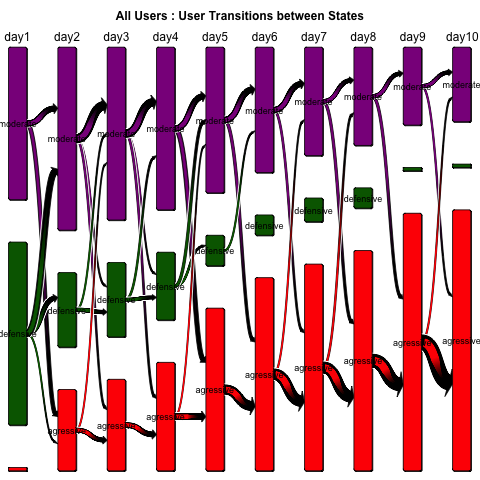
\includegraphics[width=0.8\linewidth]{transitions} 
    \caption{State transitions of all the Players at the first 10 days of installing the game.}
    \label{fig:transitions}
\end{minipage}
\quad
\begin{minipage}[b]{0.65\linewidth}
    \centering
        \begin{tabular}{ccc}
         \includegraphics[width=0.33\textwidth]{cluster1} &
         \includegraphics[width=0.33\textwidth]{cluster2} &
         \includegraphics[width=0.33\textwidth]{cluster3} \\
         \multicolumn{3}{c}{ 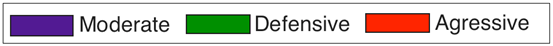
\includegraphics[width=0.75\textwidth]{legend} }
         \end{tabular}
     \caption{\label{fig:clusters} State transitions within three clusters found by our method.}
\end{minipage}
\end{figure}

%
%\begin{table}[t]
%\caption{Discovered Playing States}
%\label{tab:states}
%\centering
%\begin{tabular}{ccccccc}
%\bf State & \bf Pvp Pr. & \bf Pve Pr. & \bf Points Mean & \bf Session Mean & \bf LevelUp Pr. & \bf Pay Pr. 
%\\ \hline \\
%\texttt{Aggressive} & 0.2472  &  0.2430  &  88.10   &  4.58   & 0.1664  & 0.0031 \\  
%\texttt{Defensive}  & 0.0295  &  0.0581  &  1238.36 &  34.19  & 0.0177  & 0.0956 \\
%\texttt{Moderate}   & 0.0947  &  0.1044  &  476.22  &  12.95  & 0.0553  & 0.0320 
%\end{tabular}
%\end{table}


%\begin{figure}[t]
%\centering
%    \begin{tabular}{ccc}
%     \includegraphics[width=0.26\textwidth]{cluster1} &
%     \includegraphics[width=0.26\textwidth]{cluster2} &
%     \includegraphics[width=0.26\textwidth]{cluster3} \\
%     \multicolumn{3}{c}
%      { 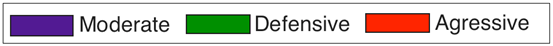
\includegraphics[width=0.45\textwidth]{legend} }
%    \end{tabular}
%     \caption{\label{fig:clusters} State transitions within the three clusters found by our method.
%              }
%\end{figure}
%
{\bf Clustering Results.} We compare the results of our clustering methods with two alternatives: Kmeans and Gaussian Mixture Model (GMM) by using a popular evaluation method based on Davis-Bouldin (DB) index \cite{dbindex} (we remind the readers that we don't have the ground truth). 
We tune the number of clusters for Kmeans using DB index, and report the one that has the best (the smallest) DB index value. 
Table \ref{tab:clustering} reports the clustering results of all methods, 
where our method outperforms the alternatives. We also plot the state transitions within each clusters  
and found that our method produces the most meaningful results. Here, we show the within cluster transitions found by our
method in Figure \ref{fig:clusters}.  




\section{Conclusion}
%%In this paper, we study the problem of clustering
%%gamer's time series.  In particular, we solved two tasks: 
%%1) identifying gamers' underlying playing states using HMH, 
%%and 2) clustering gamers' based on their state transitions using
%%a Dirichlet clustering method. 
%%We experimented on one of the strategy game developed by Zynga Inc,
%%and the results reveal interesting results that can help improve the game design.

There are many ways to cluster time series and in previous sections we reported on some of those. The specific approach we took, to first identify latent sates and then cluster the time series of the latent states, is motivated by the need to have game designers interact with the results.  There are mainly two kind interactions we aimed at: first, the results have to be interpretable by the game designers, and second we need to give game designers a way to provide side information and influence the results.  We found that by using latent states, and "naming" the latent state using the properties of the distribution of the actions they generate, the game designers and product managers could get to actionable information from the clustering.  The use of the Dirichilet process approach also provide means for them to provide side information regarding which players should and should not be in the same clusters.  We are currently studying the best ways to quantify these interactions. 




%\subsection*{Acknowledgments}

%\subsubsection*{References}
\small{
    \bibliography{draft}{}
    \bibliographystyle{plain}
}

% \subsubsection*{References}
% \small{
% [1] Alexander, J.A. \& Mozer, M.C. (1995) Template-based algorithms
% for connectionist rule extraction. In G. Tesauro, D. S. Touretzky
% and T.K. Leen (eds.), {\it Advances in Neural Information Processing
% Systems 7}, pp. 609-616. Cambridge, MA: MIT Press.

% [2] Bower, J.M. \& Beeman, D. (1995) {\it The Book of GENESIS: Exploring
% Realistic Neural Models with the GEneral NEural SImulation System.}
% New York: TELOS/Springer-Verlag.

% [3] Hasselmo, M.E., Schnell, E. \& Barkai, E. (1995) Dynamics of learning
% and recall at excitatory recurrent synapses and cholinergic modulation
% in rat hippocampal region CA3. {\it Journal of Neuroscience}
% {\bf 15}(7):5249-5262.
% }

\end{document}
